\chapter{Machine learning}
\label{chap:machineLearning}

\section{Introduction}

The field of machine learning is concerned with algorithms that ``learn" from previous experience. 
These algorithms are presented with an observed dataset and tasked with connecting descriptions of the data with some underlying quantities of interest. Machine learning algorithms typically have a high degree of flexibility, giving a considerable advantage over more traditional rule-based algorithms, particularly when the learning task is complex.
Subsequently, this class of algorithms has already been widely adopted in many areas of high energy physics, with a comprehensive review provided in Ref~\cite{ml_in_hep}.

Machine learning can broadly divided into three areas: supervised learning, unsupervised learning, and reinforcement learning. A supervised machine learning algorithm, which describes all algorithms developed in this thesis, is one in which the algorithm is presented with a set of labelled examples to learn from. The algorithm aims to tune its parameters using information from given features of the observed examples. The goal of a supervised learning algorithm is to accurately predict the label, which may be categorical or continuous, of a datum, when later presented with unseen (and potentially unlabelled) data. 

In contrast, unsupervised algorithms are provided with unlabelled data, and consequently the learning objective is typically less well defined. In general, these algorithms are tasked with learning a structure or groupings underlying the data. A common unsupervised learning task is the clustering of unlabelled data into discrete groups, usually based on some similarity metric between the population. %For example you could categorise birds based on similarity of the input data e.g. bird with a large curbed beak and wingspan greater than X should be grouped into the a single family (maybe representing an Eagle) etc.

In the final category, reinforcement learning algorithms, the algorithm is again not provided with examples of labelled data. Instead, it learns from taking exploratory actions within some environment, which are either rewarded or penalised by some external mechanism, in process similar to trial-and-error. The goal of the algorithm is to maximise the overall reward achieved by its actions. 

Since neither unsupervised or reinforcement learning techniques are used within this thesis, the remainder of this chapter pertains only to supervised learning tasks. Applications of note include the classifiers trained in the triggering system under development for the High Granularity Calorimeter CMS upgrade project (chapter~\ref{chap:detector}), the reconstruction and correction techniques for particles used in the \Hee analysis (chapter~\ref{chap:objectReco}), and in the development of analysis categories targeting both \ggH and VBF \Hee events (chapter~\ref{chap:eventCategorisation}). This chapter gives an overview of the core concepts in machine learning and discusses algorithms pertinent to later chapters of this thesis. 

\section{Concepts in machine learning}

\subsection{Problem statement}

A typical supervised machine learning problem organises the data to learn from into a vector space $X=\mathbb{R}^{m}$, where each dimension is some observable quantity often referred to as a \textit{feature}. Each element of the input feature space corresponds to a single feature vector, $\vec{x_{i}}\in X$, describing the properties of the corresponding datum. The goal of a machine learning algorithm is to construct a model, $f$, %NOTE X_I is the set/vector of observations/features of event i

$$f(\vec{x},\vec{w})\rightarrow Y,$$

\noindent that maps the input vector, $\vec{x}$, to a property of interest, $Y$, given a set of model parameters, $\vec{w}$~\cite{statistical_learning}. The property to be determined, often referred to as the label or target vector, can be continuous or categorical. This defines two types of machine learning task:

\begin{itemize}
    \item \textit{Classification tasks}, where the aim of the classifier is to predict one of $k$ possible classes,  $f(\vec{x},\vec{w})\rightarrow y$, where $y\in\{1, ..., k\}$. The simplest example is the case of a two-class prediction problem, also termed a binary classification problem, where $k=2$. Examples of binary classifiers are presented in the search for \Hee decays, where signal events resulting from true Higgs boson events form one class, and background events entering the analysis selection resulting from processes other than the signal, form the second. The number of classes is not, however, limited to two, with so-called \textit{multi-class} models developed to predict one of many possible outcomes.
    % in Section~\ref{chap:hgg}, a so-called multi-class model is developed to predict one of nine classes of ggH signal events, defined by the kinematic properties of the Higgs boson and associated final state products.
    \item \textit{Regression tasks}, where the aim of the classifier is to predict some continuously varying feature value of the data, $f(\vec{x},\vec{w})\rightarrow y$, where $y\in\mathbb{R}$. An example of a machine learning-based regression is presented in Section~\ref{subsec:elec_reco}, where the task is to predict the true value of the electron energy, from a list of features describing the reconstructed electron. 
\end{itemize}

\subsection{Model training}
\label{subsec:ML_model_training}

The development of a typical machine learning model can be divided into two phases, the first of which is \textit{training}. During the training phase, the algorithm is presented with labelled examples to learn from. The learning process involves tuning the free parameters of the model according to a \textit{loss function}, $L$. The loss function quantifies the performance of the model during training and depends both on the predicted outcomes and the corresponding true labels, aggregated in some way over the training data,

$$L(y,f(\vec{x},\vec{w})) \rightarrow \mathbb{R}.$$

\noindent The exact choice of loss function is informed by both the task to be learned and desired model properties. For regression tasks, the mean squared error is often used. For classification tasks, a typical choice is the so-called cross entropy, defined for a binary classification problem as:

\begin{equation}\label{eqn:cross_entropy}
L = -\sum_{i}[y_{i}\ln(p_{i}) + (1-y_{i})\ln(1-p_{i})],
\end{equation}

%A training using this particular loss metric is equivalent to minimising the negative log-likelihood of the correct class.%or maximising the likelihood of the correct class - https://rohanvarma.me/Loss-Functions/

\noindent where $p_{i}$ is the predicted probability for event $i$. The objective during model training is to minimise the loss with respect to the model parameters. This is typically achieved using a gradient descent-based optimisation where the loss hypersurface is descended with respect to $\vec{w}$, until reaching a global minimum of $L$,

$$\vec{\nabla}_{\vec{w}}L = 0.$$

\noindent In practice, evaluating this expression over the entire dataset is computationally costly, particularly when the number of training examples and dimensionality of the input feature space are large. Therefore, a more efficient version of the optimisation procedure, termed \textit{stochastic gradient descent} (SGD)~\cite{backprop}, is often preferred. This method makes sequential updates to the weight vector by computing the gradient on a subset of the entire training dataset. The model weights are updated as

$$\vec{w}\rightarrow \vec{w}-\eta\vec{\nabla}_{\vec{w}}L,$$

\noindent where $\eta$ is the \textit{learning rate} and controls the magnitude of weight updates. This update procedure is repeated either by cycling through the entire data in sequential batches, or by selecting batches at random, with replacement. 
Since the gradient computed in each batch will only approximate the true gradient evaluated over all training examples, the direction of descent down the loss surface will not always be optimal. However, with enough iterations, the procedure typically still converges towards the global minimum in $L$, at a much faster rate than the nominal gradient descent algorithm.

Up to now, the procedure could be viewed in the context of any gradient-based objective minimisation procedure. However, we also require the model to be capable of generalising beyond the observed training data. If the descriptive power of the model, also known at the model capacity~\cite{deep_learning}, is too large for the complexity of the problem, the model parameters will be tuned to the training data arbitrarily well, in a process known \textit{overfitting} or \textit{overtraining}. This leads to large variance in predictions if the training dataset is modified, an undesirable effect for model generalisation.
In contrast, if the descriptive power of the model is too small, it is again subject to generalisation error due to poor approximation of the underlying mapping function. In this case, the resulting model is said to be \textit{underfit}. 

To illustrate this concept, Figure~\ref{fig:ML_overfitting} shows a set of dummy observations, $y$, drawn from an underlying sinusoidal function $y=\sin({x})$, with the addition of some amount of Gaussian noise. The twenty observations are divided equally into a training set, used to tune the model parameters, and a testing set, where the performance of the model will be evaluated. The task is to fit an order-N polynomial to the training data, that also describes well the unseen test data. The loss function to be minimised for this simple fit is the mean squared error, which is also used to quantify how well the order-N polynomial fits both the training and testing data. Figure~\ref{fig:ML_overfitting} demonstrates that lower order functions, for example an order-1 polynomial, lack sufficient complexity to capture the underlying relationship between $x$ and $y$, resulting in a considerable loss on both the training and testing sets. Conversely, functions with high order, for example an order-8 polynomial, have enough flexibility to fit the training data arbitrarily well, yet generalise poorly on the unseen test data. The loss is therefore very small when evaluated on the training set, but largest of all models when computed on the test data. A balance between the two previous functions is achieved when using the medium complexity order-3 polynomial, which has enough freedom to model the underlying distribution, while remaining conservative enough to avoiding overfitting to statistical fluctuations in the training data.

To reduce the generalisation error of a model, a suitable balance between overfitting and underfitting must be drawn, commonly known as the \textit{bias-variance trade-off}. One approach to maximising the trade-off is to add additional penalties to the loss function to prevent overly-complex mapping functions being learned. These penalties, known as regularisation terms~\cite{deep_learning}, can be scaled during training to modify the strength of the regularisation. Although many types of regularisation exist, common forms add a penalty proportional to the magnitude of the model weights summed. This particular approach prevents individual weights obtaining overly large values during the training phase, a common feature of overtrained models.

\begin{figure}[htbp!]
\centering
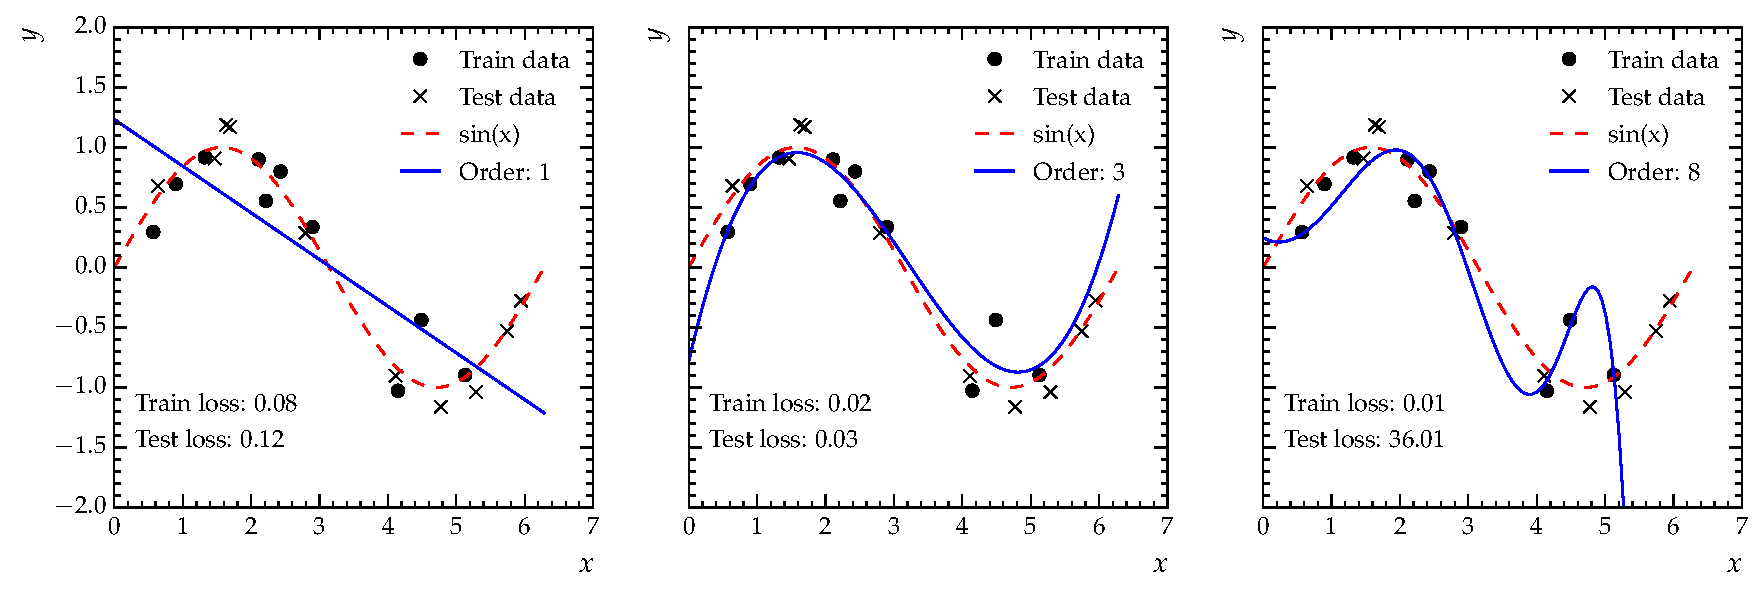
\includegraphics[width =1.0\linewidth]{Figures/ML/overfitting_example.pdf}\hfill%               
\caption[An example of underfitting and overfitting to training data with a linear regression.]{An illustrative example of underfitting and overfitting of a simple linear regression. A sample of toy data (black markers) is drawn from an underlying sinusoidal distribution, with a small amount of Gaussian noise added. The data are divided into a training set and testing set. Three polynomial fits are performed using data from the training sample: an order-1 polynomial (left), order-3 polynomial (centre), and an order-8 polynomial (right). The most simple model lacks sufficient capacity to describe the underlying distribution, resulting in a large loss (mean squared error) when evaluated on both the training and testing data. The overly-complex order-8 polynomial overfits to the Gaussian fluctuations in the training data and thus is unable to generalise well on the testing set. The order-3 polynomial provides a suitable balance between underfitting and overfitting; it describes the underlying distribution accurately, while also generalising well on the unobserved data.}
\label{fig:ML_overfitting}
\end{figure}

\subsection{Performance evaluation}

The second phase in developing a machine learning model is the evaluation step, which can be divided into two parts: the performance evaluated on a validation set, and on a test set. The validation set comprises some fraction of the dataset that is withheld from training, and instead used to tune unlearned parameters (hyperparameters) of the model. These could include regularisation coefficients, the learning rate for SGD described above, or a host of other tuneable parameters. The test set, which was already introduced in the example of Figure~\ref{fig:ML_overfitting}, comprises a fraction of the data, usually between 10 and 30\%, that remains unseen by the model during training. It is chosen to be representative of the entire distribution of the dataset. Following the training phase, the performance is evaluated on the test set to quantify both the absolute performance and the model generalisation power. A common test of generalisation is to compare the performance evaluated on both the training and testing set. For a model with good generalisation power, these should be similar; for an overtrained model, the performance on the training set is typically greater than on the unseen data.

The exact metric with which to evaluate a model is often dictated by the learning task. For classification, a standard choice is the area under the receiver operating characteristic curve~\cite{ROC_AUC} (ROC AUC). Each point on a ROC curve is populated by evaluating the true positive rate (TPR) and false positive rate (FPR) at a given threshold on the classifier output. The TPR is defined as the fraction of correctly labelled signal events, while the FPR is the fraction of background events that were incorrectly labelled as signal, at the selected threshold value.
The integral of this curve, which provides a single value to quantify performance, is 0.5 for a model that predicts a class at random, and approaches unity for a classifier performing perfect separation.
Figure~\ref{fig:ML_ROC_example} demonstrates for a simple binary classifier, how a ROC curve may be built from the distribution of model output values (or \textit{scores}) for each class.
The ROC AUC metric can also be adapted to classification tasks with more than two classes. In such cases, all but one classes are merged, and a ROC curve is generated to quantify the separation power of the merged class against the single remaining class. In this way, for a $N$-class classification problem, $N$ ROC curves are produced. Simpler metrics for evaluating the performance of multiclass models may also suffice, with a common choice being the fraction of correctly classified events, also known as the \emph{accuracy}.
For regression tasks, common evaluation metrics include the root mean squared error, or the mean absolute error, both of which offer an intuitive relation between the model predictions and associated loss. %e.g. MSE is in units of squared Y, but taking the sqrt makes it more interpretable.

\begin{figure}[htbp!]
\centering
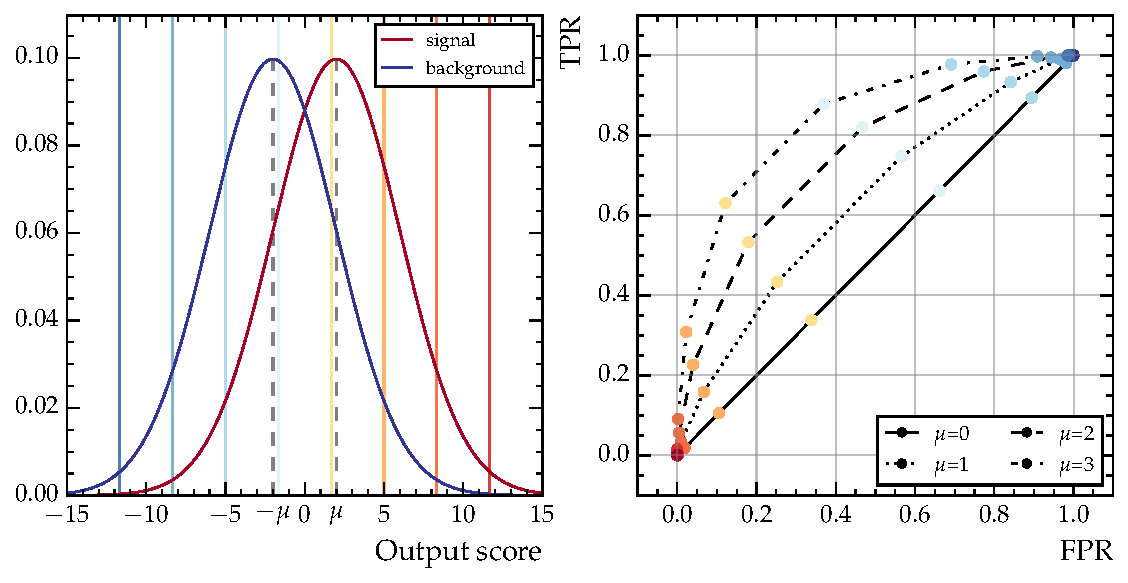
\includegraphics[width =0.95\linewidth]{Figures/ML/ROC_example.pdf}\hfill%                     
\caption[The construction of an ROC curve from the output score of a binary classifier.]{Construction of the ROC curve for a binary signal-background separation task, using the output score of a hypothetical model. Left: toy distributions of the output score are shown for the signal (red) and background (blue) classes, which are, for illustration purposes, chosen to resemble a Gaussian function symmetric about output scores of zero. The relative separation of the distributions can be parameterised using the Gaussian mean, $\mu$, which is identical in magnitude for both distributions and opposite in sign. The corresponding ROC curves are built from applying a selection on the output score (vertical lines) and computing the TPR and FPR rates. Right: resulting ROC curves, generated for different values of the Gaussian mean(s). A larger area under the curve corresponds to a larger separation between the output score distributions. Although the TPR and FPR corresponding to ten selection thresholds are drawn, a typical ROC curve is built from applying a more granular set of selections, resulting in smoother curves.}
\label{fig:ML_ROC_example}
\end{figure}



\section{Machine learning algorithms}

The landscape of possible machine learning algorithms that may be used to achieve a learning task is extremely broad.
The exact choice of algorithm is conditional on many factors including the structure and size of the input data, the desired learning outcome, and practical constraints such as the use of computational resources.
This section presents a subset of algorithms pertinent to the remainder of this thesis, namely gradient boosted decision trees (BDTs) and deep neural networks (NNs). 

\subsection{Decision trees}

To introduce gradient boosted decision trees, it is first useful to describe the construction of simple decision trees. Decision trees~\cite{DecisionTrees} perform recursive binary partitioning of the input feature space into orthogonal regions. The tree is composed of many such partitions, or nodes, each isolating a new region of input space. Nodes which terminate a branch of the tree, are labelled as leaf-nodes. Each leaf node has a value assigned to the region it isolates, which for a singular tree, corresponds to an element from the set of model predictions. For a regression task, this region holds a continuous number, whereas for classification, the region will assign probabilities to the possible class types. Figure~\ref{fig:hee_decision_tree_examples} gives an illustration of a simple decision tree that partitions a two dimensional input feature space into five mutually exclusive regions. Once the tree is formed, any new input, $\vec{x}=\{x^{(1)},x^{(2)}\}$, traverses the chain of partitions, starting at the root note and ending in a single leaf node.

\begin{figure}[htbp!]
\centering
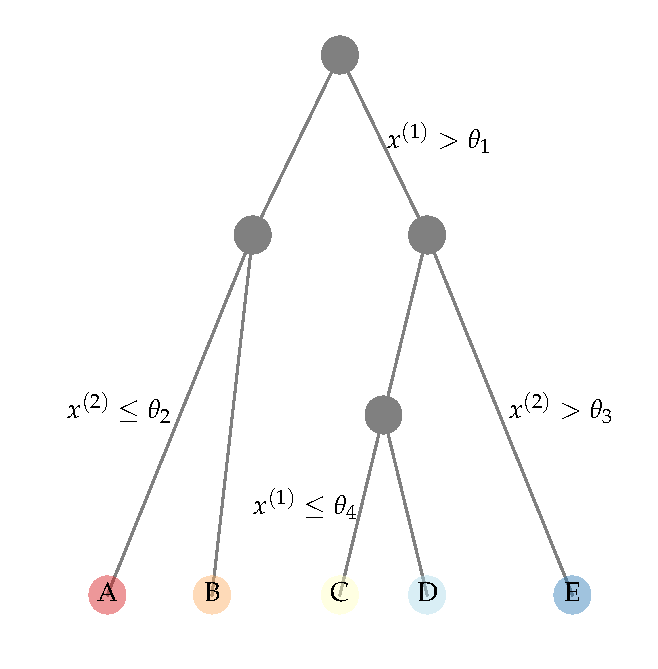
\includegraphics[width =0.45\linewidth]{Figures/ML/BDT_tree_example.pdf}\hfill%
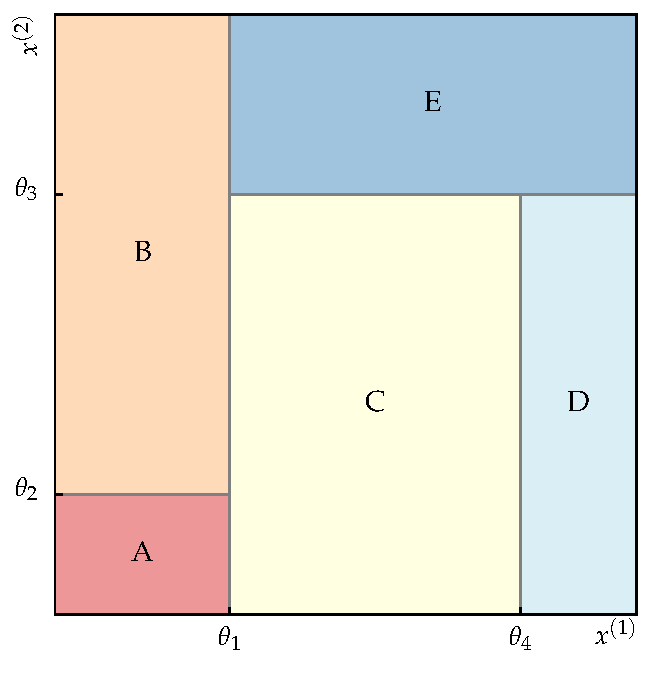
\includegraphics[width =0.45\linewidth]{Figures/ML/BDT_regions_example.pdf}\hfill%                           
\caption[The partitioning of input feature space for a decision tree with two features.]{Left: an example decision tree using two input features, $x^{(1)}$ and $x^{(2)}$. The tree makes four selections on the input features, dividing the space into five regions. Right: the partitions of the input feature space resulting from the example decision tree. Each region is mutually exclusive and typically holds some associated predicted value.}
\label{fig:hee_decision_tree_examples}
\end{figure}

The structure for a given decision tree, including which input variable is chosen at each node and the associated partition threshold, is determined during model training. Due to the computational complexity of considering all possible structures of input variables and corresponding decision thresholds, a ``greedy" optimisation is performed when growing the tree. This optimisation considers one set of partitions at a time, performing an exhaustive search over the possible variables and selection thresholds~\cite{patternRecognitionAndML}. The final choice of boundaries is chosen to maximise some measure of purity in the classification case, or minimise a measure of prediction error for regression tasks. %, for example minimising the miss-classification rate. For regression tasks, the mean-squared error is commonly used. 

When terminating the growth of a tree, common approaches are to stop adding partitions when the number of data points landing in a leaf node reaches a critical threshold, or when a predefined maximum number of partitions is reached. This typically results in large decision trees, which are then ``pruned" to prevent overfitting~\cite{patternRecognitionAndML}. Pruning is a form of regularisation, specific to decision trees, which can be achieved in many ways. One frequently used technique is to remove branches that contribute little to the overall performance of the model.

Decision tree algorithms have many advantages. They are simple, easy to interpret, and require much less computational time to train and evaluate in comparison to algorithms that result in more complex model architectures. However, the resulting models struggle to capture the mapping function for tasks where the optimal decision boundary is not somewhat aligned with the dimensions of the feature space. In addition, decision trees are prone to overfitting, if unregularised.

\subsection{Gradient boosted decision trees} 

A gradient boosted tree combines many individual decision trees in order to generate strong final predictions. 
Each individual tree is trained sequentially in order to correct the mistakes of previous ones.
This is one example of model \textit{ensembling}, where multiple base models are combined in some way to produce a committee of classifiers (or regressors), whose performance is significantly better than that of each constituent learner~\cite{weak_learners,patternRecognitionAndML}. 

Suppose that a model is to be built on a dataset $\{\vec{x}_{i},y_{i}\}$, with $i=1,2, ..., n,$ indexing the number of data points to learn from. The process to construct a gradient boosted decision tree, $F_{m}$, where $m=0,1, ..., M,$ labels the iteration of the boosting algorithm, is summarised as follows: %Note that the F's are not residuals, but the actual values of the variable being predicted

\begin{enumerate}
        
 
        \item  Train a decision tree to predict the \textit{pseudo-residuals}, defined as the set of $y_{i}-F(\vec{x_{i}})_{m-1}$. For a regression task, where the loss might be the mean squared error, this results in minimising a quantity proportional to the negative of the classical residuals (hence the name pseudo-residual). This makes clear that training to predict the negative residuals is analogous to gradient descent of the loss surface, a key insight underpinning the boosting algorithm. %More intuitively, training to minimise the pseudo residuals results in subsequent trees learning to minimise the residuals, or ``mistakes", of the previous tree.
        
        \item For each of the $j$ leaf nodes in the resulting tree, $R_{jm}$, assign a single score, $\gamma_{jm}$, that satisfies
        
        \begin{equation}\label{eqn:hee_boosting_2B}
        \gamma_{jm} = \argmin_{\gamma} \sum_{\vec{x}_{i}\in R_{jm}} L(y_{i}, F_{m-1}(\vec{x}_{i})+\gamma).
        \end{equation}
        
        
        \noindent The leaf node scores account for the previous predictions $F_{m-1}(\vec{x}_{i})$ and are computed using only $\vec{x}_{i}\in R_{jm}$. The value of $\gamma$ can be found using a line search strategy, or in some cases, solved for analytically. %For a regression problem with mean squared error loss, the values of $\gamma_{jm}$ are the average of all $y_{i}$ falling in leaf $j$. Gamma and Gamma_{jm} are the same thing in this equation, but it cant really be read left to right due to the argmin. 
        
        \item Update the predictions using
        
        \begin{equation}
            F_{m}(\vec{x_{i}}) = F_{m-1}(\vec{x_{i}}) + \eta \sum_{j}\gamma_{jm} I(\vec{x}_{i}\in R_{jm}).
        \end{equation} %i.e. update all model predictions (x) using each row x_i
        
       \noindent This step amounts to summing the predictions for each event from the current tree, with the previous predictions. The value for $\eta$ weights the predictions from all decision trees equally when summing, and can be viewed analogously to the step size, or learning rate, in gradient descent. 


\end{enumerate}

\noindent The boosting process is terminated when reaching a pre-defined maximum number of decision trees, or when successive trees fail to improve the performance by a certain threshold.


In practice, gradient boosted trees offer a significant improvement in performance over a singular decision tree, and are still relatively quick to train. The structure of each component tree is interpretable, allowing the model development to remain tractable. However, the ensemble is sensitive to the exact details of the training data, with small changes often resulting in a significantly different set of splits~\cite{statistical_learning}. In addition, given the increased model capacity, gradient boosted trees are prone to overfitting and must be carefully regularised.

\subsection{Deep neural networks}


So-called \textit{deep learning} algorithms are classes of machine learning algorithms that use artificial neural networks. Their design is partly inspired by information processing structures in biological systems. Deep networks are characterised by a large number of learnable parameters and possible configurations, resulting in complex and powerful overall structures.

The most simple of deep learning models is a multi-layer perceptron (MLP). 
A MLP comprises a collection of nodes, organised into layers, where each node is connected by weights. The vector of all such weights, $\vec{w}$, are learnable parameters fit during training. Each node receives a weighted collection of input values, which are added with one learnable bias parameter, $b$, particular to the given node. This sum is then passed through a non-linear \textit{activation function}, $f(\cdot)$, with the resulting output fed forward to the next set of nodes. The output, or activation, at each node is therefore:

\begin{equation}
    o = f\left(\sum_{i}w_{i}x^{(i)} + b\right), %stick to ^(i) being the feature indexer
\end{equation}
    
\noindent where $i$ enumerates the number of connections arriving from nodes in the previous layer. Common choices for the activation function include the rectified linear unit (ReLU), $f(\phi)=\mathrm{max}(0,\phi)$,  the sigmoid activation function, $f(\phi)=1/(1+e^{-\phi})$, and hyperbolic tangent function. In the case of the sigmoid function, the node output is identical to a logistic regression hypothesis.

Figure~\ref{fig:hee_dnn_plus_dropout} shows a network diagram for a typical MLP, which can be divided into three regions: the input, hidden, and output layers. For each training example, the input layer is simply the feature vector, with each $x^{(i)}$ connected to all nodes in the subsequent layer. The hidden layers, of which there may be many, comprise sets of fully connected (FC) internal nodes. These layers form abstract representations of the input features in a process known as \textit{automatic feature engineering}. The activations from the final hidden layer are then fed into the output layer. For regression tasks, this comprises a single node, which holds the predicted target variable. For a generic classification problem, the softmax function is commonly used at the output nodes. Outputs from softmax are given by $y_{k}=e^{a_{k}}/\sum e^{a_{j}}$, where $a_{k}$ is the input to node $k$, and $a_{j}$ is the activation for the $j^{\mathrm{th}}$ element of the output vector. The softmax function bounds node values between zero and one, allowing each output to be interpreted as a class probability.

To calculate the gradient vector, $\vec{\nabla}_{\vec{w}}=\partial L/\partial\vec{w}$, where the biases are implicitly included in $\vec{w}$, an algorithm called backpropagation~\cite{backprop} is used. At the first iteration of the algorithm, all model parameters are initialised to some starting value. Each subsequent iteration of the algorithm can be then divided into three stages:


\begin{enumerate}
    \item \textit{Forward pass}: predictions are generated for a given set of examples, referred to as a batch, by propagating each example through the network connections. The resulting loss, summed over all batch training instances, is then evaluated.
    \item \textit{Backward pass}: the gradient of the loss with respect to each learnable parameter is computed by repeated application of the chain rule. Inputs for each node, $m$, in given layer, $n$, are a function of the bias at node $m$, the activation of all weights in node $n-1$, and the weights joining to node $m$ from all nodes in layer $n-1$. This is of course true for each layer with $n>0$ in the network, and hence the gradient is propagated backwards through each one.
    \item \textit{Weight update}: after the backward pass, the gradient vector is used to update model weights using a gradient descent process.
\end{enumerate}

\noindent One complete iteration of the backpropagation algorithm, where the gradient vector has been computed and updated using all examples from the training set, is called an \textit{epoch}. Training a deep neural network typically involves many hundreds of epochs in order to reach optimal performance.

In deep learning models, the exact network structure has many non-learnable hyperparameters that can be tuned during training. These parameters often control the capacity for the network to learn the underlying mapping of input features to target vector. For example, increasing the number of hidden layers or the number of nodes in each hidden layer typically increases the model capacity. However, like any machine learning application, models with high capacity are likely to overfit; therefore, regularisation techniques specific to NNs are usually imposed. One highly effective method is \emph{dropout}~\cite{dropout}, where a random fraction of nodes are eliminated during training, as illustrated in Figure~\ref{fig:hee_dnn_plus_dropout}. This prevents the model from over-using specific neurons, and leads to \textit{effective ensembling}, where the predictions of many separate networks are aggregated during inference.

\begin{figure}[htbp!] 
\centering 
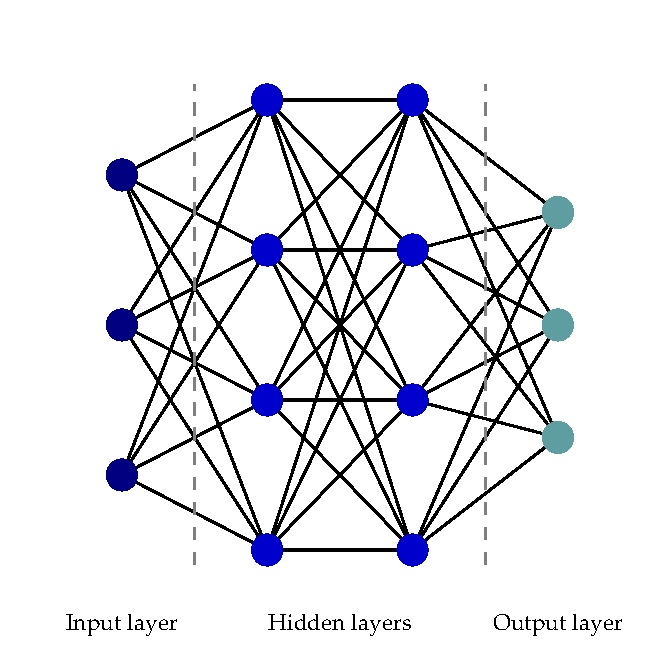
\includegraphics[width =0.46\linewidth]{Figures/ML/NNExample.pdf} \hfill
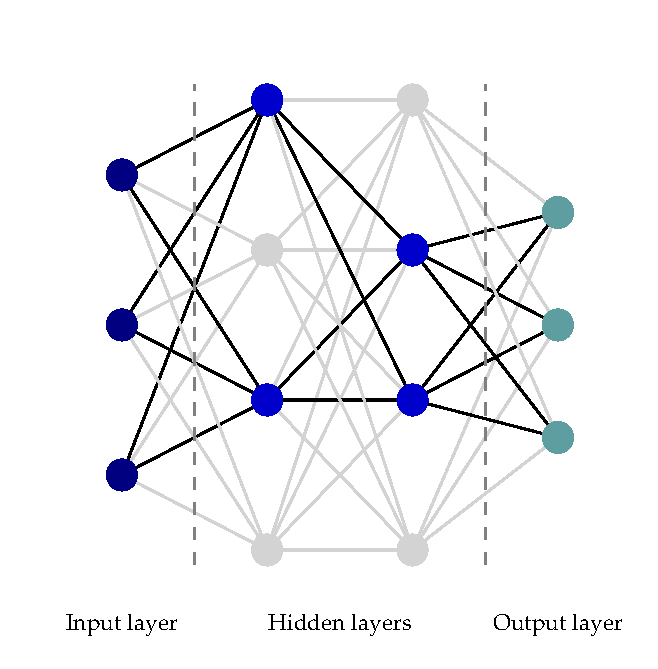
\includegraphics[width =0.46\linewidth]{Figures/ML/NNExample_dropout.pdf}
\caption[A typical neural network with dropout regularisation.]{Left: schematic of a simple feed forward NN. Nodes in the input layer hold values of the input features for each training example. These feed into layers of hidden nodes, where meaningful representations of the inputs are abstracted. The above example network is relatively shallow; deep learning models are typically characterised by having many more hidden layers. For classification tasks, the final set of nodes hold the class probabilities. For regression tasks, the network output is a single node holding the predicted value. Right: an illustration of ``dropout", a technique used to regularise NNs where a fraction of nodes and associated connections are dropped during training.}
\label{fig:hee_dnn_plus_dropout}
\end{figure}

Deep learning techniques typically produce very powerful models, with a large learning capacity. There is also less need to construct features with known predictive power (\emph{engineered} features), since this process occurs automatically within the network's hidden layers. However, deep networks typically have millions of learnable parameters that must be fit during training time. Not only does this require enormous computational power, it also obscures the learned relationship between input features and output predictions, making interpretation of the final model difficult. 

\subsubsection{Long short-term memory networks}
\label{subsubsection:lstms}

Although, thus far, only the simple case of a feed forward NN has been presented, many other variants on this structure exist. When deciding which ML algorithm to choose for a given learning task, one may appeal to the so-called \emph{inductive bias} of an algorithm~\cite{inductiveBias}, which is the set of assumptions used in the model's construction that determine how it makes predictions. For example, a linear regression assumes that the predicted variable is linearly related to the input feature values. More complex architectures make additional assumptions. For example, a convolutional neural network (CNN), which hierarchically combines input features through many filters, is well suited to classification of image data, since the assumption of correlations between neighbouring pixels in an image works well with the inductive bias of the algorithm. 

Another widely used set of ML models are recurrent neural networks (RNNs). A RNN makes assumptions similar to a CNN over a \textit{sequence} of data, motivating the organisation of inputs into list-like structures. The key feature of such a network is the repeated or recurrent propagation of previously learned information from earlier elements of the sequence, to the current element. With this view, the architecture of a RNN can be likened to a series of identical connected networks. The input to each network consists of the output from the previous network, alongside some element of the input feature sequence, as shown in Figure~\ref{fig:rnn_unrolled}. The contribution of each input is controlled through learnable weights and biases, which are tuned using the standard backpropagation algorithm on the ``unrolled" network. A typical RNN may have many recurrent layers, the last of which is fed into a feed forward network that takes the current hidden state vector to the final network output. Since a RNN is capable of propagating temporal information, typical learning tasks include speech recognition or language translation, where the input text is naturally formed from a sequence of words. However, the simple RNN implementation described above is rarely used for such tasks, since such networks often fail to capture long-range dependencies; information from earlier features of the sequence are not propagated effectively to latter parts of the network. This issue is known as the \textit{vanishing gradient problem}~\cite{vanishingGradient} and arises in cases where small weight vectors recurrently force previous networks weights to be close to zero. Since the resulting gradient vector also becomes small, the network is unable to escape this issue by updating the weight vector significantly.%less of a problem in DNNs because the weight parameter between layers can balance each other out. Leaky Relu also helps. In RNNs, the same weight matrix is used.

\begin{figure}[htbp!] 
\centering 
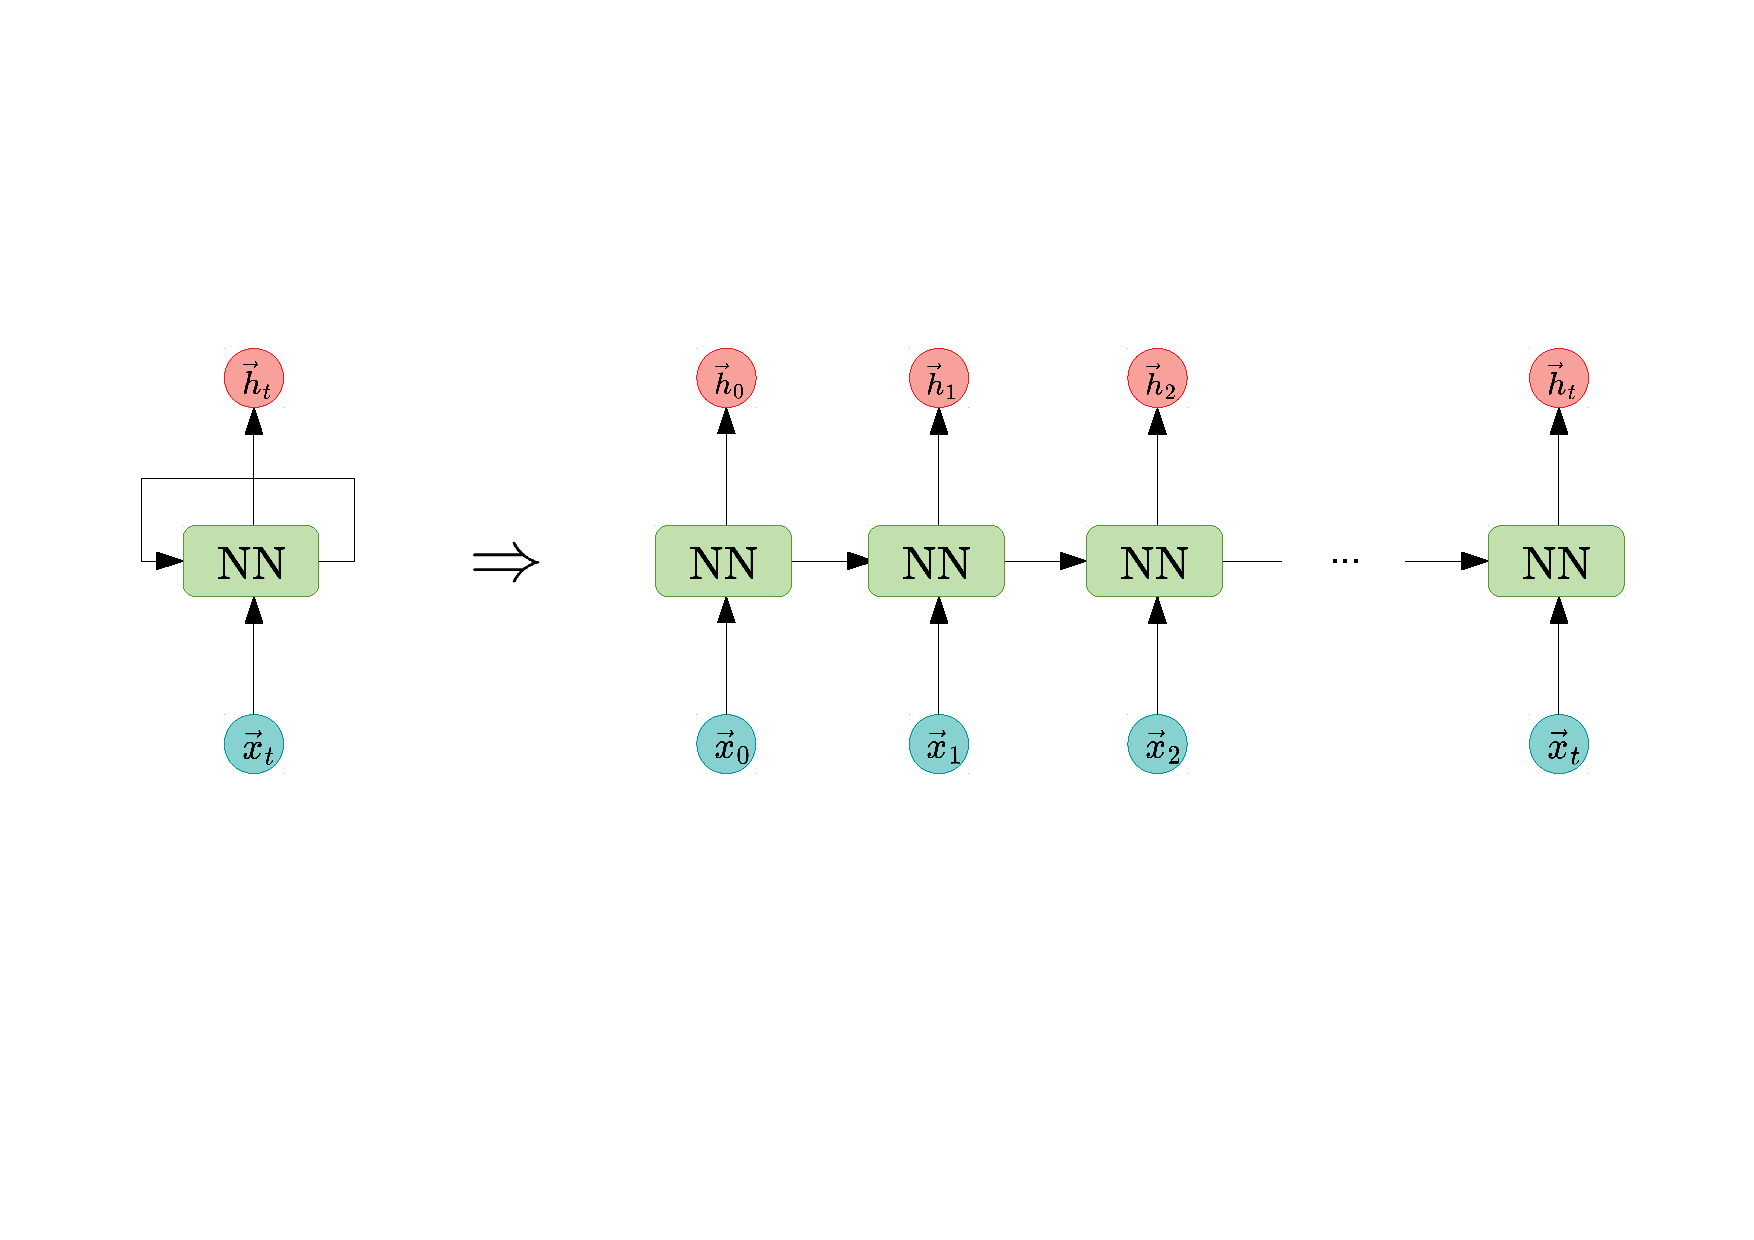
\includegraphics[trim={2cm 6cm 2cm 5cm},clip,width =0.9\linewidth]{Figures/ML/RNN.pdf}
\caption[A schematic of a recurrent neural network.]{A schematic of an ``unrolled" recurrent neural network, where the recurrent architecture is viewed as a series of connected networks (cells) propagating the hidden state forward. Inputs to each cell are an element of the input sequence, $\vec{x}_{t}$, and the previous hidden state, $\vec{h}_{t-1}$.}
\label{fig:rnn_unrolled}
\end{figure}
      

In order to solve the vanishing gradient problem, many variations on traditional RNNs have been proposed, including the long short-term memory (LSTM) network~\cite{LSTM}. As shown in Figure~\ref{fig:lstm_schematic}, an LSTM contains repeating cells with interacting components. To illustrate the function of each unit, consider an input sequence with elements, $\vec{x}_{t}$. %no need to enumerate row with the subscript (i) because we've said we're just looking at one input and it propagation to step t. so vec(x) might be a sentence, at t could be the 3rd (or t th) word in the sentence. 
The key property of each cell is the \textit{state} vector, $\vec{C}_{t}$, which for a cell observing input $\vec{x}_{t}$, can be thought of as holding learned information from all previous elements, $\{\vec{x}_{0},\vec{x}_{1}, ..., \vec{x}_{t}\}$. Each unit in the LSTM can modify the cell state using three gate mechanisms:% in what follows, t indexes the cell AND the element of the sequence, since each cell takes one element of the sequence as input. Note that x_t can be a vector itself, hence the vector notation. In our case it is a vec{x} is a vector/list of info for a single jet, and so t labels the jet number and its associated info (I think - yeah it has to be, else the order of the kinematic information INSIDE the vector would be important, which it shouldn't be. Its just like in word to vec models, where th input word is represented as a vector, and it is the relation between these vectors that carries the temporal information)

\begin{itemize}
    \item \textit{Forget gate:} this gate learns which information will be discarded from the previous cell. Inputs to this gate are $\vec{x}_{t}$, and the previous hidden state, $\vec{h}_{t-1}$. These are fed into a feed-forward NN with learnable weights, $\vec{w}^{f}$, and biases, typically using a sigmoid activation function. The resulting output can be therefore be expressed as: $\vec{o}^{f}_{t}=\sigma\left(\vec{w}^{f}\cdot[\vec{h}_{t-1},\vec{x}_{t}]\right)$, where biases have been absorbed into $\vec{w}^{f}$, and the $\sigma$ function is applied to each element in the output vector. Elements in the previous cell state are updated through the point-wise multiplication $\vec{o}^{f}_{t} \cdot \vec{C}_{t-1}$. This can be viewed as a learnable filter for the previous state --- elements multiplied by values close to zero are forgotten, while values close to one are remembered and propagated onward.
    %point wise meaning dot product here, not vector/matrix multiplication. Point wise since it needs to be the same dimension as the cell state. Its like placing a filter over a (hidden state+x_t) vector which blurs out/removes some of the values. Hence why we need sigmoid (0,1) for EACH output node of the network. Each node has a sigmoid applied to it basically, creating a vector to overlay on the hidden state. Conversely, tanh just does "squeezing". Note that [h,x] is just another vector of x appended to h really i.e. the input vector to this NN. In an example tasks of predicting the next words in a sentence, the overall cell state might consider the gender of the present subject at x_{t}, and so may try to forget previously seen genders based on this new information.
    \item \textit{Input gate:} the aim of this gate is to control the information added to the current cell state. This section is composed of two units, each taking as input $[\vec{h}_{t-1},\vec{x}_{t}]$. The first unit learns to filter which values of the current cell state should be updated, passing inputs through a feed forward NN with sigmoid activation, to give output: $\vec{o}^{\,i}_{t}=\sigma\left(\vec{w}^{i}\cdot[\vec{h}_{t-1},\vec{x}_{t}]\right)$. The second unit creates a vector of new candidate values, $\Tilde{\vec{C}}_{t}$, used to update the state, using a similar network with $\tanh(\cdot)$ activation, yielding the output: $\Tilde{\vec{C}}_{t}=\tanh\left(\vec{w}^{C}\cdot[\vec{h}_{t-1},\vec{x}_{t}]\right)$. Combining with the \textit{forget gate}, this results in the updated cell state: $\vec{C}_{t} = \vec{o}^{f}_{t}\cdot \vec{C}_{t-1} + \vec{o}^{\,i}_{t}\cdot\Tilde{\vec{C}_{t}}$
    %why tanh not sigmoid? Its zero centred and so long sum operations distributions the gradients better i.e. equal negative and equal positive in general. In the example of the sentence prediction, we would want to add the gender of the new subject to the cell state, and replace the old one to be forgotten. Sigmoid output says which values of update, tan output gives the actually updates to the elements of the vector.
    \item \textit{Output gate:} finally, the hidden state, which is also passed to the next cell, must be updated. Firstly, a NN with sigmoid activation is used to filter the previous hidden state information, to be passed on. This is combined with $\tanh(\vec{C}_{t})$ in pointwise multiplication, where the hyperbolic tangent ensures each element in the current cell state spans the range $\{-1,1\}$. Along with $\vec{C}_{t}$, this hidden state is passed to cell $t+1$, which has an identical structure of gates formed from independent learnable weights and biases. %in the langauage task, we might want to output info relevant to a verb, in case thats what coming next e.g. whether the subject is singular or plural so we know how the verb should be conjugated
\end{itemize}

\noindent Many variants on the gated cell structure exist, including most notably the gated recurrent unit model, which combines the \textit{input} and \textit{forget} gate into a single update step~\cite{GRUs}. However, for many leaning tasks, the resulting performance is typically unaffected by the exact choice of recurrent algorithm~\cite{LSTMPerformances}.
%if you take the derivative of the weights, the function has a lower dependence on W so helps mitigate vanishing gradient problem

\begin{figure}[htbp!] 
\centering 
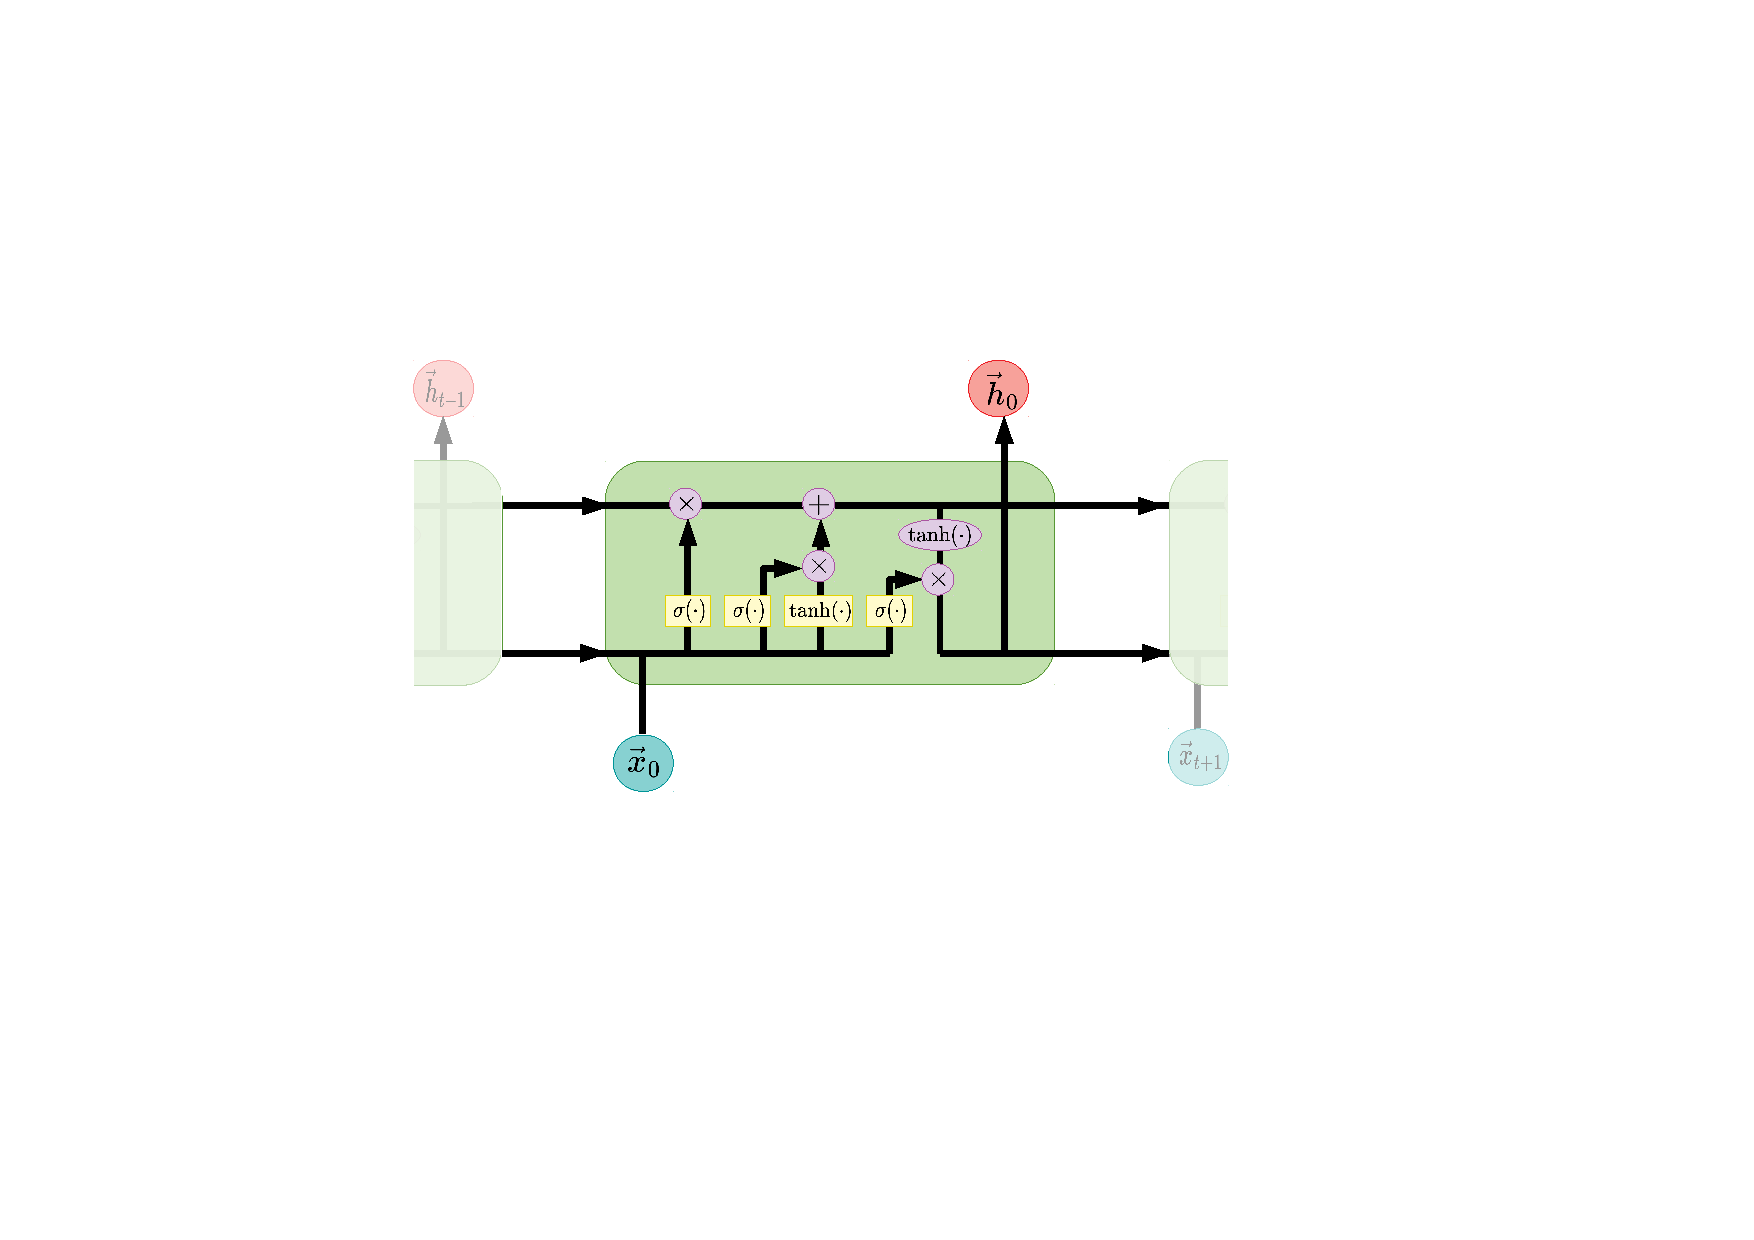
\includegraphics[trim={5.5cm 6cm 7cm 5cm}, clip, width =1\linewidth]{Figures/ML/LSTM_cutaway.pdf}
\caption[A schematic of an LSTM neural network.]{Schematic of the repeating module inside an LSTM deep neural network, a variant on the traditional RNN. Each cell is composed of a \textit{forget gate}, \textit{input gate}, and \textit{output gate}, which regulate the flow of information to and from the overall cell state. Inputs to each cell are an element of the input sequence, $\vec{x}_{t}$, and the previous hidden state, $\vec{h}_{t-1}$. Yellow boxes indicate neural network layers, where all output nodes are transformed either by a sigmoid or hyperbolic tangent function, although hidden layer activations may differ. Purple circles indicate point-wise addition or multiplication.}
\label{fig:lstm_schematic}
\end{figure}
      
%So in our case, our sequence is the three jet vectors, and each cell takes one of the individual vectors of jet values i.e. t goes from 1 to 3. In the HP opt we can have multiple LSTMs, stacked vetically and hence multiple cell states and outputs.
      
\section{Summary}      

A supervised machine learning algorithm is one that learns to perform a desired task through observation of many labelled examples. The parameters of the model are adjusted with the aim of jointly maximising the performance on the learning task and the generalisation capabilities on unobserved data. Although these models may require dedicated tuning of their unlearned parameters, they typically offer a considerable improvement in performance over rule-based approaches. As a result, these models have been widely applied in particle physics~\cite{ml_in_hep}. The machine learning models trained in this thesis include shallow learning architectures, which are interpretable and lightweight to train, such as the boosted decision tree performing e/$\gamma$ identification in the CMS Level-1 Trigger (L1T) phase-2 upgrade (chapter~\ref{chap:detector}). Deep learning models are also explored, including a LSTM NN used in categorisation of VBF \Hee events (chapter~\ref{chap:eventCategorisation}). In contrast to shallower architectures, these models have a large number of learnable parameters resulting in resource-heavy trainings. Their implementation, optimisation details, and performance comparisons are left to later chapters.
